\section{Approche numérique}

\subsection{Transport avec une direction fixée pour $\vec{v}$}
\begin{frame}{Equation de transport - Discrétisation}

  \begin{block}{Equation de transport}
    \begin{equation*}
      \frac{\partial w(\vec{r}, \theta, \phi, t)}{\partial t} = -\vec{v} \cdot \nabla w(\vec{r}, \theta, \phi, t) - M v w(\vec{r}, \theta, \phi, t) + 
      w_{sce}(\vec{r}, \theta, \phi, t)
    \end{equation*}
    
    \begin{columns}[c]
      \begin{column}{5cm}
        \begin{itemize}
        \item $\vec{r} : (x_1,...,x_{dim})$ \\
          1D,2D, ou 3D en espace
        \end{itemize}
      \end{column}
      \begin{column}{5cm}
        \begin{itemize}
        \item $\vec{v} : (\theta, \phi)$ \\
          2D pour les directions
        \end{itemize}
      \end{column}
    \end{columns}

    \begin{center}
      \textcolor{red}{Modèle 5D instationnaire}
    \end{center}
  \end{block}

  \begin{alertblock}{Discrétisation : Schéma différence finies implicite centré}
    \begin{columns}[c]
      \begin{column}{6cm}
        \begin{equation*}
          \frac{\partial w}{\partial t} = \frac{w^{t+1}_{\vec{r}} - w^t_{\vec{r}}}{\Delta t}
        \end{equation*}
      \end{column}
      \begin{column}{6cm}
        \begin{equation*}
          \frac{\partial w}{\partial x_i} = \frac{w^{t+1}_{r_i + 1} - w^{t+1}_{r_i - 1}}{2\Delta x_i}
        \end{equation*}
      \end{column}
    \end{columns} 

  \end{alertblock}

\end{frame}

\begin{frame}{Schéma aux différences finies}
  \begin{equation*}
    \frac{w_{\vec{r}}^{t+1} - w_{\vec{r}}^{t}}{\Delta t} + 
    \sum \limits_{i=1}^{Dim} v_i \left( \frac{w_{r_i+1}^{t+1} - w_{r_i-1}^{t+1}}{2 \Delta x_i} \right)
    + Mvw_{\vec{r}}^{t+1} = w_{sce}
  \end{equation*}

  %forme matricielle
  \begin{columns}[c]
    \begin{column}{5cm}
      \centering
      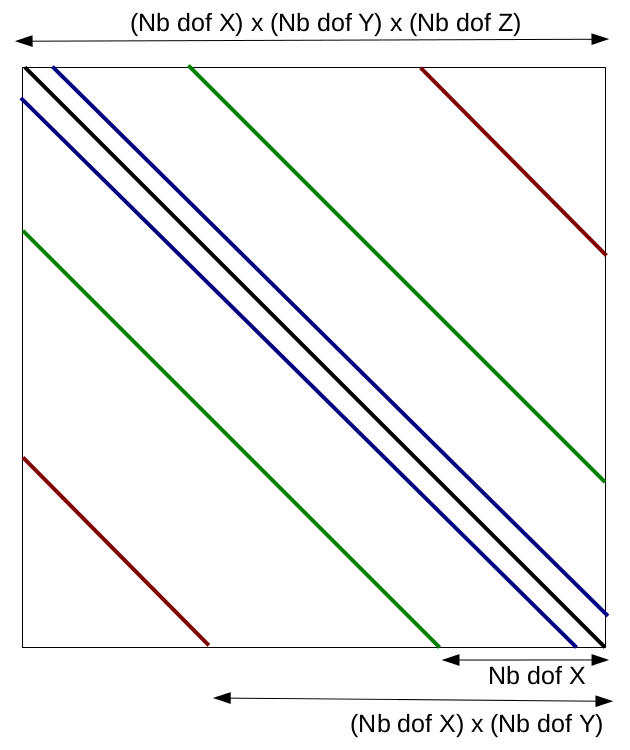
\includegraphics[scale=0.3]{Figures/FD_matrix.png}
    \end{column}
    \begin{column}{6.5cm}
      \begin{itemize}[label=$\rightarrow$]
      \item \textcolor{black}{$\bullet$} terme diagonal : $\frac{1}{\Delta t} + Mv$
      \item \textcolor{blue}{$\bullet$} schéma centré en $x$ : $\pm \frac{v_x}{2\Delta x}$
      \item \textcolor{green}{$\bullet$} schéma centré en $y$ : $\pm \frac{v_y}{2\Delta y}$
      \item \textcolor{red}{$\bullet$} schéma centré en $z$ : $\pm \frac{v_z}{2\Delta z}$
      \end{itemize}
    \end{column}
  \end{columns} 

\end{frame}

\begin{frame}
  Video 1D Dirichlet homogene sans stabilisation
\end{frame}

\begin{frame}{Stabilisation : ajout d'un terme de diffusion artificiel}
  %Stabilisation : ajout d'un terme de diffusion artificiel
  \vspace*{-0.6cm}
  \begin{eqnarray*}
    \frac{\partial w(\vec{r}, \theta, \phi, t)}{\partial t} &=& -\vec{v} \cdot \nabla w(\vec{r}, \theta, \phi, t) - M v w(\vec{r}, \theta, \phi, t) + 
    w_{sce}(\vec{r}, \theta, \phi, t) \\
    &+& \text{ \textcolor{red}{$\nabla (\tau_{art} \nabla w(\vec{r}, \theta, \phi, t))$} } 
    \qquad \tau_{art} = \frac{\rho h \prod \limits_{i=1}^{Dim} v_i }{\parallel \vec{v} \parallel}
  \end{eqnarray*}

  %avec $\tau_{art} = \frac{\rho h \prod \limits_{i=1}^{Dim} v_i }{\parallel \vec{v} \parallel}$

  \vspace*{-0.3cm}
  %forme matricielle
  \begin{columns}[c]
    \begin{column}{4.5cm}
      \centering
      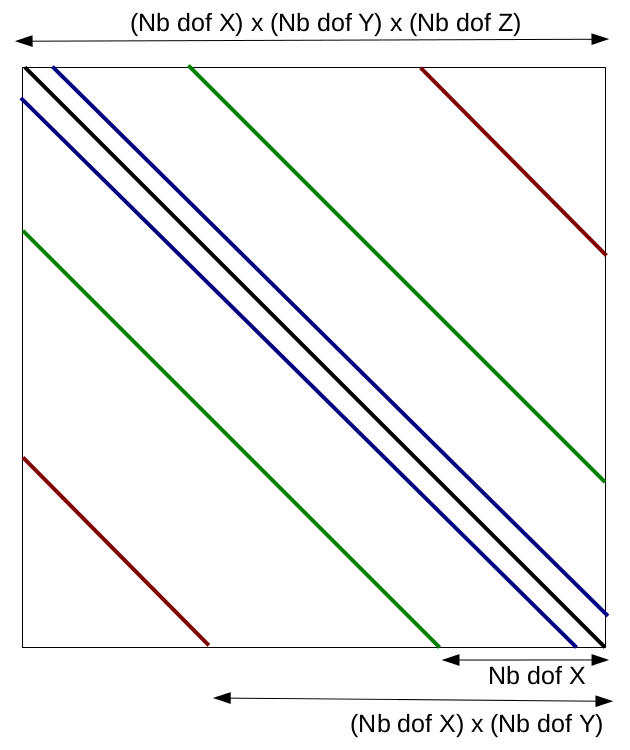
\includegraphics[scale=0.26]{Figures/FD_matrix.png}
    \end{column}
    \begin{column}{7.5cm}
      \begin{itemize}[label=$\rightarrow$]
      \item \textcolor{black}{$\bullet$} terme diagonal : $\frac{1}{\Delta t} + Mv$ 
        + \textcolor{red}{$\frac{2\tau_{art}}{\Delta x^2} + \frac{2\tau_{art}}{\Delta y^2} + \frac{2\tau_{art}}{\Delta z^2}$}
      \item \textcolor{blue}{$\bullet$} schéma centré en $x$ : $\pm \frac{v_x}{2\Delta x}$
        - \textcolor{red}{$\frac{\tau_{art}}{\Delta x^2}$}
      \item \textcolor{green}{$\bullet$} schéma centré en $y$ : $\pm \frac{v_y}{2\Delta y}$
        - \textcolor{red}{$\frac{\tau_{art}}{\Delta y^2}$}
      \item \textcolor{red}{$\bullet$} schéma centré en $z$ : $\pm \frac{v_z}{2\Delta z}$
        - \textcolor{red}{$\frac{\tau_{art}}{\Delta y^2}$}
      \end{itemize}
    \end{column}
  \end{columns} 

\end{frame}

\begin{frame}
  Video 1D Dirichlet homogene avec stabilisation
\end{frame}

\subsection{Prise en compte de la condition limite}
\begin{frame}{Condition aux limites}

  Sur les bords du domaine (= murs de la salle) :
  \begin{itemize}[label=$\bullet$]
  \item une partie de l'énergie est réfléchie de façon spéculaire %(probabilité $1-d$)
  \item l'autre partie est réfléchie de façon diffuse %(probabilité $d$) \\
    \vspace*{0.2cm}
  \item $R$ (coefficient de réflexion) et $d$ (coefficient de diffusivité) dépendent de la paroi considérée
  \end{itemize}

  \vspace*{-0.4cm}
  \begin{small}
    \begin{equation*}
      w(\vec{r},\theta,\phi,t) = \underbrace{R(1-d)w(\vec{r},\hat{\theta},\hat{\phi},t)}_{\text{reflexion spéculaire}}
      + \underbrace{ \int_{0}^{2\pi} \int_{0}^{\frac{\pi}{2}} Rd\frac{1}{\pi v} \vec{v}'w(\vec{r},\theta',\phi',t) sin \theta' d\theta' d\phi'}_{\text{reflexion diffuse}}
    \end{equation*}
    si $\vec{v} \cdot \vec{n} < 0$ ( $w(\vec{r},\theta,\phi,t)$ = 0 sinon) \\
  \end{small}

  où $\vec{v} \cdot \vec{n} = -\hat{\vec{v}} \cdot \vec{n}$, avec
  \begin{equation*}
    v=
    \left(
    \begin{array}{lll}
      cos(\theta)\\
      sin(\theta)cos(\phi)\\
      sin(\theta)sin(\phi)
    \end{array}
    \right)
    \Rightarrow
    \left \{
    \begin{array}{ll}
      \hat{\theta} = \pi - \theta \\
      \hat{\phi} = \pi - \phi \\
    \end{array}
    \right.
  \end{equation*}
  et $\vec{v} \cdot \vec{n} \neq -\vec{v}' \cdot \vec{n}$
\end{frame}

\subsection{Transport prenant en compte plusieurs directions pour $\vec{v}$}
\begin{frame}{Stratégie}

  \begin{columns}[c]
    \begin{column}{6cm}
      \begin{itemize}[label=$\bullet$]
      \item Directions $(\theta,\phi)$ organisées selon une grille 2D
      \item Resolution 3D pour chaque direction $(\theta,\phi)$
      \item \textbf{Résultat} : somme des densités dans toutes les directions :\\
        $w(\vec{r},t) = \sum \limits_{(\theta,\phi)} w(\vec{r},\theta,\phi,t)$
      \end{itemize}

      \begin{alltt}
        for[ pas de temps $t$ ] \\        
        \hspace*{0.2cm} for[ direction $(\theta,\phi)$ ] \\
        \hspace*{0.4cm} assemblage matrice
        \hspace*{0.4cm} assemblage second membre
        \hspace*{0.4cm} Resolution $\Rightarrow w(\vec{r},\theta,\phi,t)$
        \hspace*{0.4cm} $w(\vec{r},t)$ += $w(\vec{r},\theta,\phi,t)$
      \end{alltt}
    \end{column}
    \begin{column}{6.5cm}
      \begin{figure}[H]
        \centering
        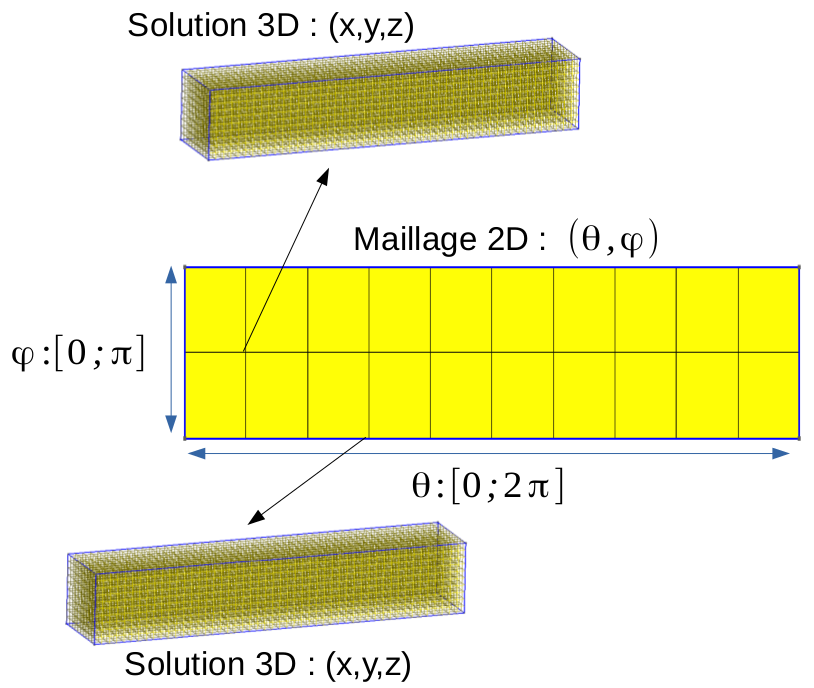
\includegraphics[scale=0.32]{Figures/Schema_mesh.png}
      \end{figure}
    \end{column}
  \end{columns}
\end{frame}

